\section{Redox-Reaktionen}
Redox = \emph{Red}uktion - \emph{Ox}idation \\
Bsp. Verbrennung, Photosynthese, Korrosion, ... \\

Redox-Reaktionen sind Elektronenübertragungs-Reaktionen.
\begin{figure}[htbp]
	\centering
	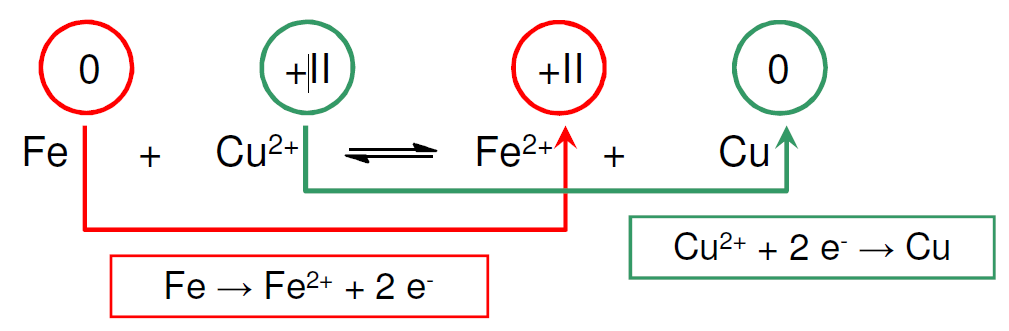
\includegraphics[width=0.6\linewidth]{images/9_Redox_Reaktion.png}
\end{figure}

Oxidation: Abgabe von $e^-$ $\Rightarrow$ Erhöhung der Oxidationszahl \\
Reduktion: Aufnahme von $e^-$ $\Rightarrow$ Erniedrigung der Oxidationszahl \\

Reduktionsmittel = Elektronenspender, Oxidationsmittel = Elektronenakzeptor


\subsection{Oxidationszahlen}
Oxidationszahlen (OZ) sind eine Hilfsgrösse um Redoxreaktionen zu beurteilen. Sie werden mit römischen Ziffern geschireben. \\
Regeln:
\begin{enumerate}
	\item Die OZ der Atome in ihrer elementaren Form ist 0, Bsp. $O_2$, $Na$
	\item Bei einatomigen Ionen entspricht die OZ der Ionenladung, Bsp. $Na^+$: OZ=+I
	\item Bei Molekülen werden die Bindungselektronen dem elektronegativerem Atom zugeordnet. Faustregeln: $F$ immer -I, $O$ fast immer -II, $H$ fast immer +I
	\item Die Summe aller OZ muss der Ladung des Teilchens entsprechen.
\end{enumerate}

\subsection{Die Redox-Reihe}
Die Redox-Reihe gibt Auskunft über die Stärke eines Stoffs als Reduktions- bzw. Oxidationsmittels. Eine Redox-Reaktion kann ablaufen, wenn das Reduktionsmittel höher in der Tabelle liegt als das Oxidationsmittel.\\

Tabelle siehe Anhang. \\